%29/01 - Fátima Sánchez Cabo
\chapter{Diseño experimental y principios estadísticos del análisis de datos ómicos}
El transcriptoma permite estudiar cómo se expresan los ARNs, incluyendo tanto ARNs codificantes (como los ARNm) como no codificantes (como microARNs, ARN de transferencia, etc.). El proteoma se centra en el estudio de las proteínas, que son los productos funcionales de muchos ARNm. Finalmente, el metaboloma estudia los metabolitos, que son los productos finales de las reacciones bioquímicas en las células.

\begin{figure}[h]
\centering
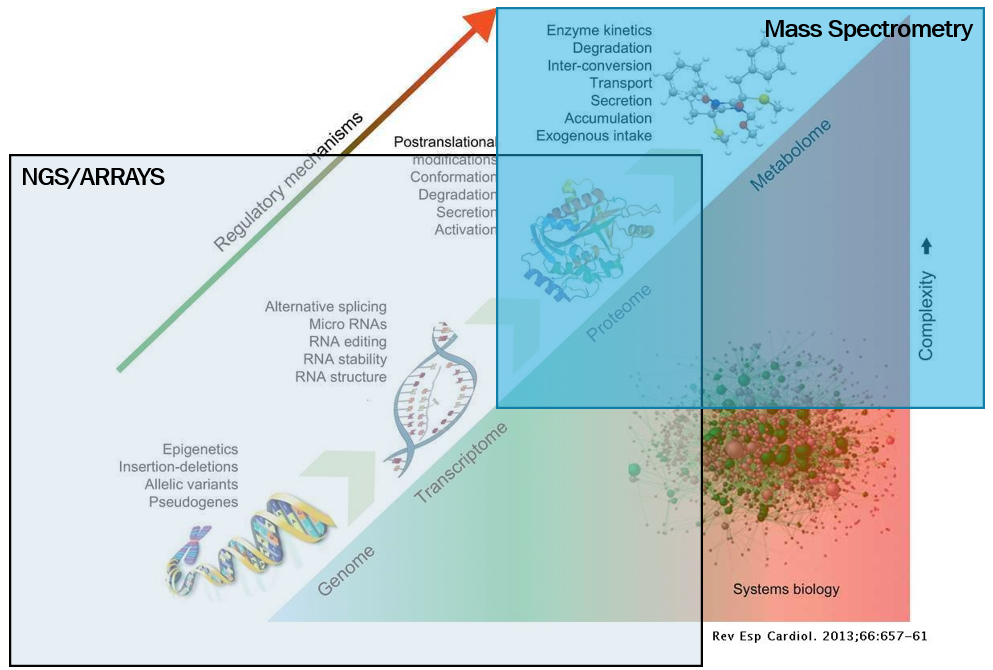
\includegraphics[width = 0.6\textwidth]{figs/omics.png}
\end{figure}

La genómica, transcriptómica y proteómica se pueden analizar utilizando tecnologías de secuenciación de próxima generación (NGS) y microarrays. Sin embargo, la proteómica y la metabolómica también se estudian comúnmente con espectrometría de masas, una técnica que permite identificar y cuantificar moléculas basándose en su masa y carga. Aunque la espectrometría de masas ofrece un mayor detalle en la identificación de proteínas y metabolitos, la secuenciación es más escalable y se está popularizando, especialmente en estudios a gran escala. Dos empresas comerciales que permiten la secuenciación de proteínas son Olink y Somalogic.

\section{Pipeline de un experimento ómico}
El pipeline de un experimento ómico aplica tanto a la cuantificación de la expresión génica con NGS, como a la identificación de proteínas con espectrometría de masas o de metabolitos con espectrometría. El proceso generalmente sigue los siguientes pasos:
\begin{enumerate}
\item \textbf{Pregunta biológica}: Todo experimento ómico comienza con una pregunta biológica clara. Esta pregunta debe ser lo suficientemente específica para guiar el diseño experimental y la elección de la plataforma tecnológica. Por ejemplo, si la pregunta es sobre la expresión génica en una cohorte grande de pacientes, la secuenciación de ARN (RNA-seq) podría ser la opción más adecuada.
\item \textbf{Elección de la plataforma tecnológica}: La elección de la tecnología (NGS, espectrometría de masas, microarrays, etc.) debe basarse en la pregunta biológica y no al revés. Por ejemplo, si se busca un alto rendimiento y escalabilidad, la secuenciación podría ser preferible sobre la espectrometría de masas.
\item \textbf{Diseño experimental}: Es crucial diseñar el experimento de manera que se minimice el sesgo y se maximice la reproducibilidad. Esto incluye la selección adecuada de controles, la replicación biológica y técnica, y la consideración de factores de confusión.
\item \textbf{Adquisición de datos}: Una vez diseñado el experimento, se procede a la recolección de datos. Esto puede implicar la secuenciación de ARN, la identificación de proteínas por espectrometría de masas, o la cuantificación de metabolitos.
\item \textbf{Preprocesamiento de datos}: Los datos crudos suelen requerir un preprocesamiento que incluye la corrección de errores, la normalización y la eliminación de ruido. Este paso es crucial para asegurar que los datos sean de alta calidad antes de proceder al análisis.
\item \textbf{Análisis de datos}: El análisis de datos en estudios ómicos generalmente incluye:
\begin{itemize}
\item \textbf{Identificación de genes diferencialmente expresados}: Esto implica comparar los niveles de expresión génica entre diferentes condiciones (por ejemplo, tejido sano vs. tejido enfermo) para identificar genes que están regulados al alza o a la baja.
\item \textbf{Análisis de clusters}: Este método agrupa genes o muestras con patrones de expresión similares, lo que puede ayudar a identificar subtipos de enfermedades o vías biológicas relevantes.
\item \textbf{Ingeniería reversa de redes génicas}: Este enfoque intenta reconstruir las redes de regulación génica a partir de los datos de expresión, lo que puede proporcionar insights sobre cómo los genes interactúan entre sí.
\end{itemize}
\item \textbf{Estandarización y almacenamiento de datos}: Los datos deben ser estandarizados y almacenados en bases de datos públicas o privadas para su posterior acceso y análisis. Una base de datos importante es el \textit{Gene Expression Omnibus (GEO)}, que alberga datos de expresión génica de diversos organismos y condiciones experimentales.
\item \textbf{Integración e interpretación biológica}: Finalmente, los datos se integran con información biológica adicional (como anotaciones funcionales, interacciones proteína-proteína, etc.) para interpretar los resultados en un contexto biológico más amplio. Esto puede llevar a la identificación de biomarcadores, dianas terapéuticas o mecanismos moleculares subyacentes a una enfermedad.
\end{enumerate}

\section{Diseño experimental}
El diseño experimental es esencial en estudios ómicos debido al alto coste de los experimentos. El objetivo es minimizar el coste y maximizar la información obtenida. Para lograrlo, hay dos aspectos clave:
\begin{enumerate}
\item \textbf{Pregunta biológica:} Es imprescindible tener una pregunta biológica clara y específica. Esto determina si el enfoque es \textit{data-driven} (exploratorio) o \textit{hypothesis-driven} (basado en hipótesis).
\item \textbf{Conocimiento de la tecnología:} Es crucial entender las limitaciones y capacidades de la tecnología utilizada. Esto incluye la precisión de las mediciones, la replicación y la identificación de variables que pueden introducir sesgos o variabilidad técnica. 
\end{enumerate}

En un experimento, hay dos tipos de errores:
\begin{itemize}
\item \textbf{Errores aleatorios:} No son predecibles, pero se pueden minimizar mediante la repetición de las mediciones.
\item \textbf{Errores sistemáticos:} Son predecibles y se pueden eliminar mediante la normalización o calibración de los datos.
\end{itemize}

Los principios para minimizar errores son:
\begin{enumerate}
\item \textbf{Replicación:} Incluye réplicas técnicas (para minimizar errores aleatorios) y réplicas biológicas (para asegurar que los resultados sean extrapolables a la población). La distinción entre réplicas biológicas y técnicas depende de qué fuentes de variación se estudien o, alternativamente, se consideren fuentes de ruido. Existen las réplicas técnicas, las cuales minimizan los errores aleatorios mediante el promedio y ayudan a testar la tecnología, y réplicas biológicas, que permiten sacar conclusiones extrapolables a la población completa y no solo del individuo, además de poder controlar la variabilidad en diferentes pasos experimentales.
\item \textbf{Randomización:} Asegura que las muestras sean representativas de la población.
\item \textbf{Blocking:} Reduce fuentes conocidas de variación que no son relevantes para la pregunta biológica.
\end{enumerate}

\subsection{Ejemplo de diseño experimental}
Supongamos que se mide la expresión de un gen en células de hígado de ratón, pudiendo realizar solo 48 mediciones. Se pueden considerar tres fuentes de variabilidad:
\begin{itemize}
\item \textbf{Replicación biológica}: se utilizan varios ratones, habiendo variabilidad entre los diferentes animales.
\item \textbf{Replicación entre biológica y técnica}: se escogen varias células de cada raón.
\item \textbf{Replicación técnica}: se realizan varias mediciones de cada célula. Las distintas mediciones de una misma célula deberían ser similares.
\end{itemize}
Si se realiza la media de los tres ratones, la medida va a ser muy variable en relación con una sola medida, pero esto sirve para el test estadístico, ya que son medidas independientes. En caso de tener medidas dependientes, no se puede utilizar la variabilidad para estudiar la significancia, ya que son medidas repetidas. 

Como en este modelo propuesto hay que cuantificar la variabilidad, se pueden realizar simulaciones para determinar el número óptimo de réplicas biológicas y técnicas para minimizar la variabilidad y maximizar la precisión.

\begin{figure}[h]
\centering
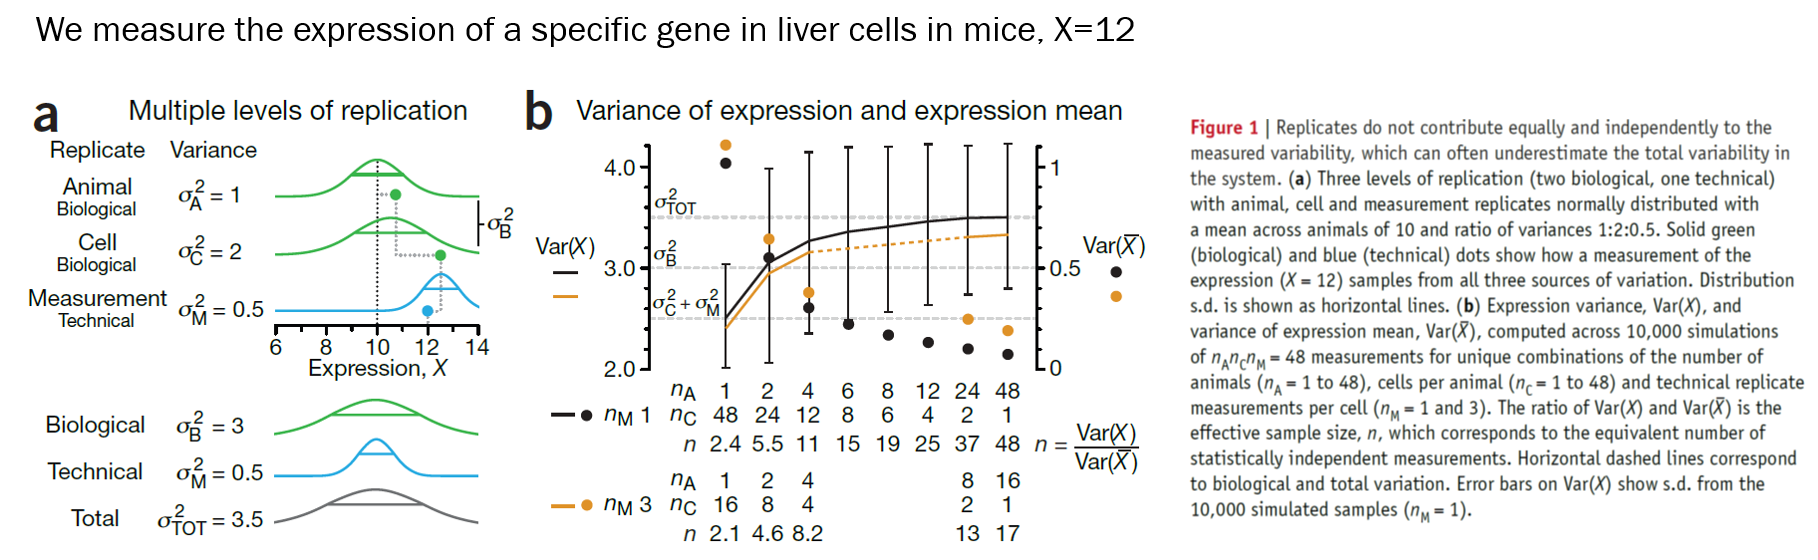
\includegraphics[width = \textwidth]{figs/replicates.png}
\end{figure}

En este experimento de ómicas, la expresión de un gen de células de hígado de ratón se cuantifica en 12. Las tres fuentes de variabilidad (animal, célula y medición) suman un 3,5. Las normales están centradas en 10, ya que las medidas están saliendo en ese valor, no en 12. Hay más variabilidad biológica que técnica, transformando las gaussianas en una campana más aplastada. Se realizaron simulaciones cambiando el número de animales, el número de células y el número de réplicas técnicas. Se hacen 10.000 asignaciones, para que se agrupen de forma diferente las combinaciones del número total (48 animales, 1 sola célula; 24 animales, 2 células; ...; 1 animal, 48 células). Sabiendo la cantidad de animales, células y mediciones, se puede sacar el tamaño muestral real del experimento, permitiendo calcular así la diferencia entre la variabilidad experimental y la variabilidad real. En ómicas, somos poco capaces de estimar la variabilidad, ya que en general hay pocas réplicas. Si esto después de mete en un t-test, y la variabilidad es muy pequeña (o incluso 0), entonces el resultado es muy grande, teniendo un p muy pequeño, rechanzando la hipótesis nula de que no hay diferencia en la expresión.

Para tecnologías ómicas, se deben incluir al menos 3 réplicas biológicas. Todo esto es para la experimentación con animales. En caso de experimentación en humanos, la variabilidad es gigante. 

\subsection{Réplicas vs profundidad}
Cuando comenzó la secuenciación, cuanto más se secuencie, más caro es el experimento. Por tanto, ¿es mejor más réplicas a menos profundidad, o menos réplicas a más profundidad? Hubo varios estudios con muchas simulaciones que vieron que lo importante era la secuenciación con réplica biológica. El número de lecturas tiene algo de relevancia, pero llegados a un número, no compensa a hacer mucha más secuenciación porque se llega a un plateau en cuanto a genes diferencialmente expresados. Las métricas aumentan más teniendo varias réplicas biológicas que teniendo varias lecturas. 

\begin{figure}[h]
\centering
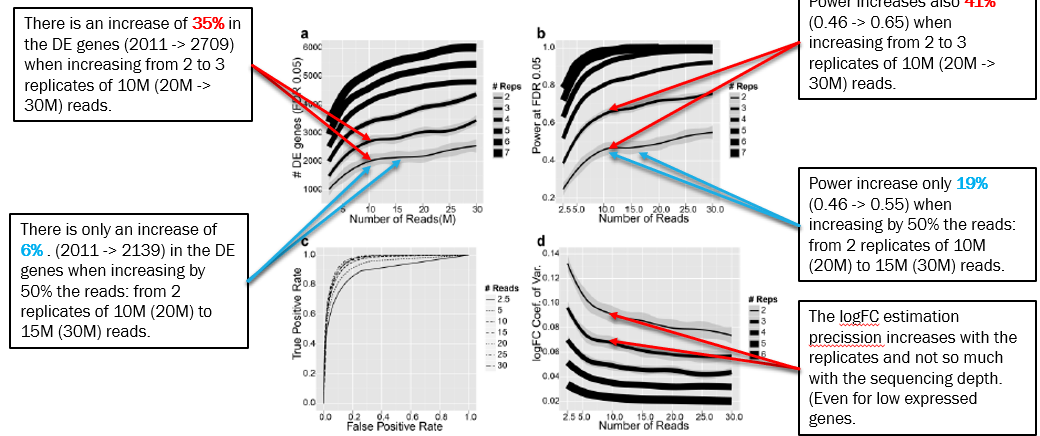
\includegraphics[width = \textwidth]{figs/replicates-depth.png}
\end{figure}

\subsection{Pooling, batch y blocking}
En el contexto de los experimentos ómicos, el \textbf{pooling} es una estrategia que consiste en combinar (o "agrupar") múltiples muestras biológicas en una sola muestra antes de realizar el análisis. Esta técnica se utiliza principalmente para reducir costes y simplificar el procesamiento de muestras, especialmente cuando se trabaja con un gran número de individuos o cuando los recursos económicos son limitados. En lugar de analizar cada muestra individualmente, se mezclan varias muestras en una sola. Por ejemplo, si tienes 12 muestras de ARN de diferentes individuos, podrías combinarlas en 3 grupos (pools) de 4 muestras cada uno. Una vez combinadas, las muestras agrupadas se procesan y analizan como una sola. Esto significa que, en lugar de obtener datos individuales para cada muestra, obtienes un resultado promedio para cada pool. En el caso de muestras humanas no se hace porque se pierde información individual fenotípica y genotípica, pero en animales sí puede ser una buena idea si las características específicas por especimen (sexo, camada, edad, etc.) no son relevantes para el experimento. Lo mejor es tener cuantas más réplicas independientes posibles. 

\begin{figure}[h]
\centering
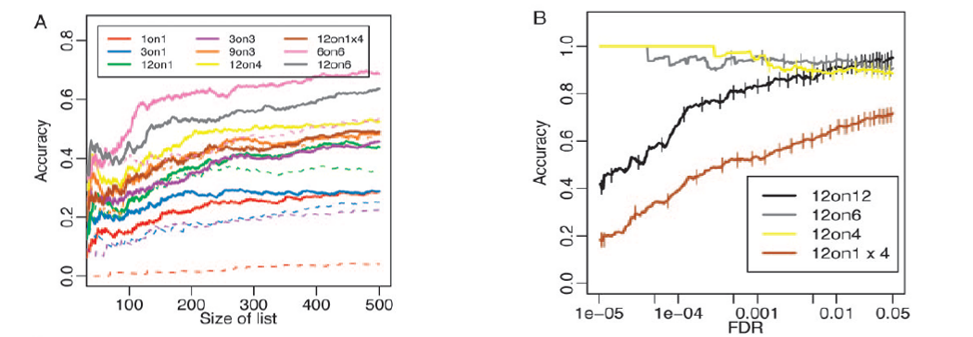
\includegraphics[width = 0.9\textwidth]{figs/pooling.png}
\end{figure}

Algunos pasos en los que se introduce variabilidad en NGS son:
\begin{itemize}
\item Técnica: extracción del ARN, preparación de la librería, flow-cell, barcode, científico
\item Biológica: sexo, camada/familia, edad
\end{itemize}
Además, hay sesgos sistemáticos y ruido por errores aleatorios.

Cuando los experimentos se realizan en varias tandas (por ejemplo, por ser estudios muy grandes con muchas muestras), es crucial controlar el \textbf{efecto de batch} \marginpar[\footnotesize !!!!!]  \ para evitar sesgos técnicos. Esto se puede lograr mediante la randomización de muestras entre batches y el uso de modelos estadísticos mixtos.
Nunca hay que confundir el batch con el grupo biológico relevante, ya que es imposible ver si las diferencias son debidas al grupo biológico o a la variabilidad técnica. Cuando hay condiciones biológicas muy fuertes, a veces no se ven, pero si se hacen todas las muestras de una condición en un mismo batch, probablemente se estén magnificando las diferencias observadas. Por tanto, no hay que medir las distintas condiciones biológicas en batches distintos, si no mezclar en un batch muestras de distintas condiciones biológicas para poder utilizar la variable batch en el modelo estadístico mixto, normalizando por las diferencias entre los batches.

\begin{figure}[h]
\centering
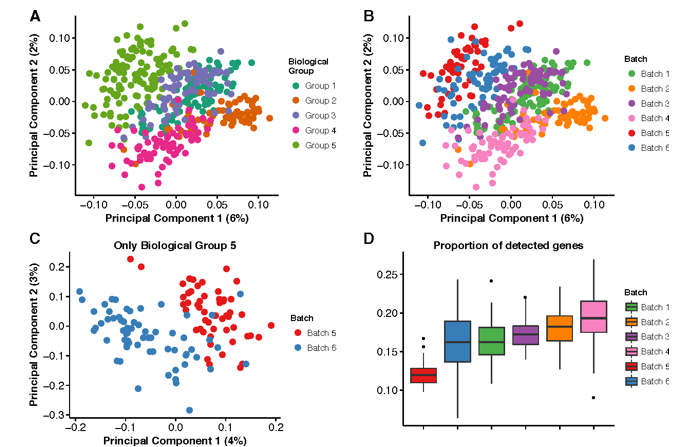
\includegraphics[width = 0.7\textwidth]{figs/batch.png}
\end{figure}

El \textbf{blocking} reduce fuentes conocidas e irrelevantes de variación entre unidades, permitiendo una precisión mayor en la estimación de las fuentes de variación estudiadas. Minimiza el efecto de variables de tipo biológico o técnico, que no son relevantes para la pregunta biológica. Una forma de hacer blocking secuenciando es metiendo adaptadores para hacer un barcoding de cada muestra, preparar la librería con todo junto y crear, de esa muestra, las distintas alícuotas a secuenciar. De esta forma se reduce el efecto de línea.

\begin{figure}[h]
\centering
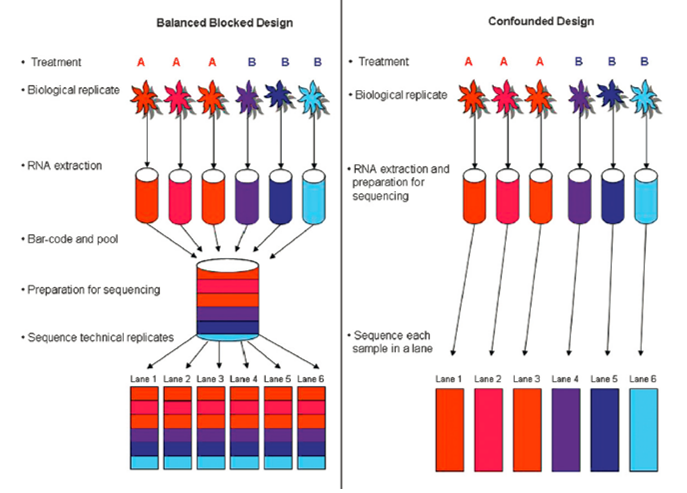
\includegraphics[width = 0.5\textwidth]{figs/blocking.png}
\end{figure}

\subsection{Diseño experimental - Ejercicios}
\subsubsection{Ejercicio de animales}
Tenemos un ratón knock-out en la proteína Bmi1. Para cada camada tenemos varios ratones WT y KO. Queremos encontrar metabolitos cuya expresión cambie significativamente entre condiciones
Disponemos de 6 camadas con el siguiente número de animales:
\begin{table}[h]
\centering
\begin{tabular}{c | c c}
Camada & KO & WT \\ \hline
L1 & 1 & 2 \\
L2 & 2 & 2 \\
L3 & 1 & 1 \\
L4 & 1 & 3 \\
L5 & 2 & 3 \\
L6 & 3 & 2 
\end{tabular}
\end{table}

\begin{itemize}
\item \textbf{Caso 1: No hay limitación económica}: se secuencia todo, ya que cuantas más muestras independientes, mejor.
\item \textbf{Caso 2: Se pueden secuenciar un máximo de 6 muestras}: De las 6 camadas se escogen aleatoriamente 3, de las cuales escoger un ratón KO y uno WT. Otra opción es coger las camadas 2 y 3 y secuenciar todos esos individuos. En este caso, como las camadas tienen efecto, se podría elegir un individuo de cada camada y hacer pool de 2 en 2. 
\item \textbf{Caso 3: L5 no tiene ningún animal KO y seguimos con el máximo de 6 muestras}: L5 no se tendría en cuenta porque podría introducir sesgos (quizás el KO no ha salido, o quizás no es viable), y del resto de camadas se escogen 3 camadas al azar para seleccionar un ratón de cada condición. Esto se debe a que no se podría comparar el pool entre la misma camada con pool entre distintas camadas.
\item \textbf{Caso 4: máximo de 6 muestras si no hay efecto de la camada}: se mezclan todos los ratones de las distintas camadas, separando por condición biológica, y se sacan 3 de cada uno al azar. Se podrían coger 12 y 12 y pooles de 4, o 6 y 6 y pooles de 2.
\end{itemize}

\subsubsection{Ejercicio de humanos}
Tenemos una cohorte de 100 muestras humanas con diabetes. Queremos probar en ellas un fármaco y ver sus efectos en la expresión génica. Podemos secuenciar un total de 40 muestras. Por estudios piloto sabemos que el sexo y el IMC afectan al impacto del fármaco. La composición de la cohorte es la siguiente:
\begin{table}[h]
\centering
\begin{tabular}{c | c c}
 & Hombres & Mujeres \\ \hline
IMC alto & 40 & 20 \\
IMC bajo & 20 & 20
\end{tabular}
\end{table}
Además, no podemos procesar todas las muestras juntas, tenemos que hacerlo en dos ejecuciones.
\begin{itemize}
\item \textbf{Q1: ¿Cómo se asignan los pacientes a los grupos fármaco y placebo?} Se escogen 5 personas de cada condición (sexo y BMI) para fármaco y otros 5 para placebo. 
\item \textbf{Q2: ¿Qué pacientes se secuenciarían en cada turno?} Se cogen ordenadamente una muestra de cada grupo y condición.
\end{itemize}

\section{Consideraciones estadísticas para datos ómicos}